\documentclass[lettersize,journal]{IEEEtran}
\usepackage[T1]{fontenc}
\usepackage{amsmath,amssymb,amsfonts,graphicx,booktabs,cite,url,textcomp}
\usepackage{tikz}
\usepackage[hidelinks]{hyperref}
\usetikzlibrary{arrows.meta,positioning,calc}
\graphicspath{{../python/latest/biotin_20260913/}}
\newcommand{\supp}[1]{\href{SPR_smart_stop_supplement.pdf}{Supplement~#1}}
\begin{document}
\title{SPR Virtual Sensor for Early Stopping: Arrival-Aware Kinetic Forecasting and Experimental Bulk-Corrected Response Analysis}
\author{Rodrigo T. Ara\'ujo, Mateus S. Marques,
Arthur A. Melo, and Antonio M. N. Lima
\thanks{\raggedright VIRTUS-CC, Department of Electrical Engineering, Universidade Federal de
Campina Grande, Campina Grande, Brazil. E-mail:
\{rodrigo.araujo,mateus.marques\}@ee.ufcg.edu.br;
\{arthur.aprigio,amnlima\}@dee.ufcg.edu.br.}
\thanks{\raggedright This work has been partially funded by SmartSens Base Systems,
VIRTUS-CC, with resources from PPI HardwareBR of MCTI, grant 055/2023,
signed with EMBRAPII.}}


\markboth{SPR Virtual Sensor for Early Stopping}{Ara\'ujo \textit{et al.}}
\maketitle

\begin{abstract}
Reducing reagent exposure in surface plasmon resonance requires
distinguishing surface-response stabilization from bulk refractive-index
drift and delayed delivery. This work presents a surface plasmon resonance virtual sensor that
combines exponential-tail forecasts with the bulk-corrected response
derivative and total-internal-reflection delivery markers.
Stopping requires stable forecasts and sustained corrected-response
stationarity. Evaluation with measured serial-flow
biotinylation sensorgrams shows a 21--62\% reduction in a baseline noise
metric and resolves a 2.19--2.26 min inter-channel delivery delay.
In one physical channel, cancellation between surface plasmon resonance and weighted total-internal-reflection slopes
reveals near-stationarity obscured in the individual signals.
Apparent time constants span 1.92--4.23 min, although sensitivity to the
fitting window limits forecast reliability.
Four-readout estimation averages 36.6 ms per update on the benchmark laptop,
supporting streaming at the measured acquisition rate. A separate
experiment tests a 25-min programmed exposure selected from the largest
reference-run point forecast of 23.92 min. Its measured post-rinse response
provides an experimental outcome at the selected duration, without
refitting the kinetic model. Local-exposure and baseline analyses qualify
the comparison with the reference and distinguish retained response from
quantitative endpoint equivalence.
\end{abstract}
\begin{IEEEkeywords}
Bulk compensation, experimental early stopping, kinetic time constant,
serial flow, surface plasmon resonance, virtual sensor.
\end{IEEEkeywords}
\section{Introduction}
Surface plasmon resonance (SPR) sensorgrams combine surface-associated
changes with bulk refractive-index variation, delivery and noise. For early
stopping, a raw-angle plateau is unnecessary: a corrected signal can
become stationary while SPR and TIR continue to drift. Conversely,
stationarity alone does not establish a retained layer. Transport,
heterogeneity and changing solution conditions confound kinetic
interpretation\cite{schuck}.

Early stopping requires an estimate of the remaining surface response
together with a criterion for preserving the intended experimental
outcome. Kinetic forecasts must therefore be interpreted in relation to
local reagent delivery and the response retained after solution exchange.
This study evaluates a virtual-sensor approach that combines optical
signal processing, delivery markers and response derivatives with
model-based forecasting. Experimental sensorgrams provide the basis for
assessing both predictive performance and retained-response consistency.

Recent work reinforces the separation between optical processing, kinetic
inference and experimental design. Svirelis et al. demonstrated that bulk
correction must account for the sensing-layer geometry\cite{bulk2022}.
Nguyen et al. combined initialization search and identifiability analysis
for a bivalent SPR model\cite{nguyen2023}. Gaudreault et al. showed
that kinetic inference from heterogeneous mixtures benefits from known
total concentrations and measurements across multiple
mixtures\cite{gaudreault2021}.
Mixed-phase and competitive-chaser assays show that reliable association
and dissociation measurements may require distinct experimental
configurations\cite{quinn2025,chaser2025}. These studies motivate calibrated
inputs and model qualification here; their mechanisms and performance
are not transferred to this surface-preparation experiment.

This article is a technical extension of our proceedings
paper\cite{melo2026}, which introduced an SPR virtual sensor based on
recursive nonlinear least squares (NLLS) and asymptotic forecasting.
Its software layer translates optical measurements into inferred kinetic
quantities and a forecast of the time to near-equilibrium. The present
extension retains this model-based sensing objective and the 1:1 kinetic
model as an interpretable reference. It adds experimental qualification of
the optical input, local delivery timing and a corrected-response slope
check; it does not replace the virtual sensor with signal smoothing alone.
The extension also adds a second-sensor test and new computational
benchmarks. Additional model derivations are provided in \supp{S1}; earlier
accuracy and reagent-saving claims are not transferred.



\section{Physical Model and SPR Virtual Sensor}
\subsection{Forward model and inferred quantities}
The physical forward chain separates kinetic evolution, optical layer
properties and angular readout:
\begin{equation}\label{eq:forwardcorrected}
\begin{aligned}
 C_j(t)&\xrightarrow{K}\Gamma_j(t)\xrightarrow{O}\{d_j(t),n_j(t)\},\\
 \{d_j,n_j,n_{b,j}\}&\xrightarrow{H}
 \{\Delta\theta_{\mathrm{SPR},j},\Delta\theta_{\mathrm{TIR},j}\},\\
 R_j&=\mathcal B_{S_j}[\Delta\theta_{\mathrm{SPR},j},\Delta\theta_{\mathrm{TIR},j}]\\
 &=\Delta\theta_{\mathrm{SPR},j}-S_j\Delta\theta_{\mathrm{TIR},j}.
\end{aligned}
\end{equation}
The bulk index $n_{b,j}$ enters the optical readout alongside the surface
layer. The correction operator $\mathcal B_{S_j}$ is part of the observation
chain: the virtual sensor fits $R_j$, not the uncompensated SPR shift.
Residual bulk error, nonspecific response and drift can remain. Independent
calibration of this correction matters even with a correct kinetic
model\cite{bulk2022}.
Here $C_j$ is local reagent concentration, $\Gamma_j$ is fractional surface
coverage, and $d_j,n_j$ describe the effective layer. Under the reference
reaction-limited, homogeneous 1:1 model,
\begin{equation}\label{eq:langmuir}
 \dot\Gamma=k_aC(1-\Gamma)-k_d\Gamma,\qquad d=d_{\max}\Gamma.
\end{equation}
These assumptions require experimental qualification. A local optical
approximation gives $R=\alpha d$, with sensitivity $\alpha$ distinct from
the bulk coefficient $S$. The experimental fits use this response-level
model, not a newly calibrated inversion of thickness and refractive index.
The full optical operator is given in \supp{S1}.

For constant $C$, define
\begin{equation}
 k_{\mathrm{obs}}=k_aC+k_d,\quad \tau=k_{\mathrm{obs}}^{-1},\quad
 R_{\mathrm{eq}}=R_{\max}\frac{k_aC}{k_{\mathrm{obs}}}.
\end{equation}
The 99\% target is an operational fraction of fitted response, not a
confidence level or evidence of complete site occupation. Reversible 1:1
chemistry is not established for this reagent/surface experiment.

\subsection{Implemented model and time-varying delivery}
The reported estimates use a constant-rate exponential tail with free
offset and amplitude. Changing prefix estimates do not establish a
physically varying $\tau$. The broader implementation includes delivery,
transport and additional surface states, but those models did not generate
the reported experimental rates. A delivery-aware 1:1 extension would use
\begin{equation}
 \dot\Gamma_j=k_aC_j(t)(1-\Gamma_j)-k_d\Gamma_j,
 \quad \tau_{\rm rel,j}(t)=[k_aC_j(t)+k_d]^{-1}.
\end{equation}
Dispersion can alter sensorgram curvature\cite{quinn2019}. When $C_j(t)$
changes, the equilibrium also moves, so a single $4.605\tau$ generally
does not predict 99\% completion during exchange. TIR supplies
refractive-index arrival markers, not calibrated active-reagent
concentration. Delivery time, instantaneous relaxation and fitted tail
time are therefore distinct (derivation in \supp{S1}).

\subsection{Inverse model, forecasting and operational decision}
At each observation prefix $n$, the virtual sensor estimates parameters
from the data available so far,
\begin{equation}
 \widehat{\boldsymbol\eta}_n
 =\arg\min_{\boldsymbol\eta}\sum_{i\in\mathcal W_n}
 [R_i-h(T_i;\boldsymbol\eta)]^2.
\end{equation}
The conference implementation used recursively initialized NLLS in kinetic
coordinates. The experimental tail analysis here uses
$\boldsymbol\eta=(b,A,k_{\mathrm{obs}})$ with bounded nonlinear least squares
and multiple rate initializations. Updating a prefix estimate is distinct
from actuating a valve; Section~\ref{sec:runtime} measures the desktop
estimation kernel separately from a complete instrument deployment. Figure~\ref{fig:virtual} shows the retained virtual
sensor and the experimental additions.

\begin{figure*}[t]\centering
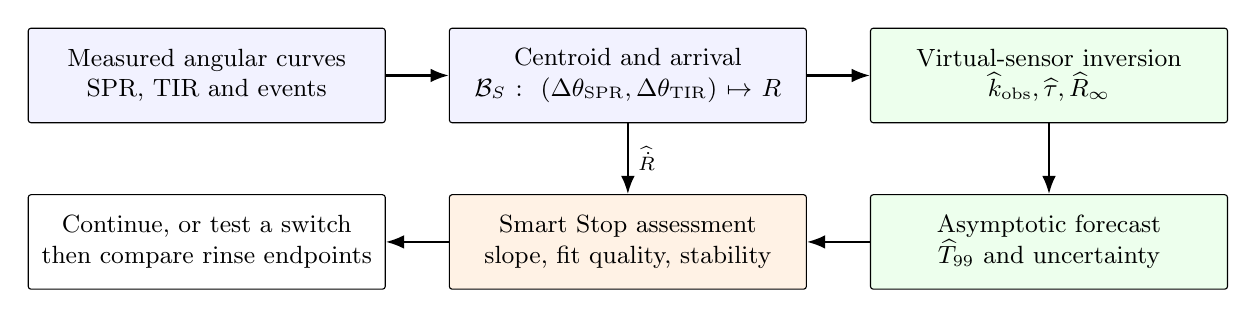
\begin{tikzpicture}[>=Latex,font=\small,
 box/.style={draw,rounded corners=1pt,align=center,minimum height=12mm,text width=43mm},
 link/.style={->,thick}]
\node[box,fill=blue!5] (input) {Measured angular curves\\SPR, TIR and events};
\node[box,right=8mm of input,fill=blue!5] (clean) {Centroid and arrival\\$\mathcal B_S:\ (\Delta\theta_{\rm SPR},\Delta\theta_{\rm TIR})\mapsto R$};
\node[box,right=8mm of clean,fill=green!7] (inverse) {Virtual-sensor inversion\\$\widehat k_{\rm obs},\widehat\tau,\widehat R_\infty$};
\node[box,below=9mm of inverse,fill=green!7] (forecast) {Asymptotic forecast\\$\widehat T_{99}$ and uncertainty};
\node[box,left=8mm of forecast,fill=orange!10] (gate) {Smart Stop assessment\\slope, fit quality, stability};
\node[box,left=8mm of gate] (outcome) {Continue, or test a switch\\then compare rinse endpoints};
\draw[link] (input)--(clean);\draw[link] (clean)--(inverse);
\draw[link] (inverse)--(forecast);\draw[link] (forecast)--(gate);
\draw[link] (clean)--node[right,font=\scriptsize] {$\widehat{\dot R}$} (gate);
\draw[link] (gate)--(outcome);
\end{tikzpicture}
\caption{SPR virtual sensor and its experimental extension. The forward
kinetic--optical model supplies the inverse model; measured optical data
supply its inputs. Parameter estimates and forecasts are virtual-sensor
outputs. Processing/arrival and corrected-slope checks extend the
conference architecture. Switching and retained-endpoint equivalence
remain to be prospectively tested.}
\label{fig:virtual}
\end{figure*}

The historical Smart Stop monitors changes in the forecast,
$|\widehat T_{99,n}-\widehat T_{99,n-q}|/(T_n-T_{n-q})$, and freezes a future
schedule after its stability conditions hold. The proposed extension also
checks the derivative of the corrected response itself. Forecast stability
and response stationarity answer different questions and neither alone
certifies a preserved post-rinse endpoint.

\subsection{Identifiability and forecast sensitivity}
A single constant-concentration association trace identifies at most an
apparent rate and response amplitude. Many pairs $(k_a,k_d)$ share the
same $k_{\rm obs}=k_aC+k_d$, and practical identifiability also depends on
noise and observation duration\cite{nguyen2023}. Neither $k_a$, $k_d$ nor
affinity is inferred here. Rate overestimation produces an earlier
forecast and larger remaining response; \supp{S1} derives that sensitivity.

\subsection{Injection clock and local exposure clock}
All reported Biotin times use $T=t-t_{\rm inj}$, so $T=0$ is reagent
insertion into the system. Local arrival occurs at $T=a_j$ in channel $j$,
and local elapsed exposure is $s_j=T-a_j$. A tail fit beginning at $T_{0,j}$
therefore forecasts
\begin{equation}\label{eq:commandforecast}
 \widehat T_{99,j}=T_{0,j}+\ln(100)\widehat\tau_j.
\end{equation}
The operator uses $T$ to schedule the repeat injection; the model uses
local arrival to interpret the response. A valve switch at $T_s$ precedes
rinse arrival by a delivery delay. Consequently, stopping the injection
clock and ending molecular contact are distinct events.

\subsection{Delivery-aware stopping criterion}
Events define intended phases; TIR identifies observed exchange and
serial delay; the corrected response estimates surface-sensitive change
on each local exposure clock. The stopping decision combines slope
equivalence with a stable tail prediction, fit quality and a practical
remaining-response margin. For a valid exponential,
\begin{equation}
 R_\infty-R(t)=\tau\dot R(t).
\end{equation}
A small slope may therefore leave appreciable remaining response when
$\tau$ is large or uncertain. Slope and rate estimates share data and are
not independent evidence. A wrong bulk coefficient can also create
apparent cancellation; stationarity is not proof of equilibrium or
successful surface coupling.

The target outcome is retained response after a matched rinse. A
prospective evaluation must fix calibration, baseline, endpoint window
and equivalence margin, verify delivered exposure, and repeat both
conditions on comparable sensors. Switching to rinse and stopping a pump
with reagent still present produce different exposure conditions. The
delivery convolution and expanded rationale are given in \supp{S1,S4}.

\section{Experimental Setup and Analysis}\label{sec:experiment}
\subsection{Acquisition and trace mapping}
Two serial-flow experiments were performed on a BioNavis MP-SPR 210A at
$10\,\mu$L/min, using water, PBS and Biotin reagent. Angular scans were
sampled approximately every 8 s. Physical channel 1 provides L1 (670 nm)
and L2 (785 nm); channel 2 provides L3 (670 nm), L5 (785 nm), L6 (850 nm)
and L7 (980 nm). Readouts sharing a channel are not independent replicates.
In both records channel 2 responds before channel 1; temporal ordering is
measured rather than inferred from the channel numbers.

The first run is the development reference; the second used a nominal
25-min injection. The experimenter confirmed the same reagent preparation,
flow rate and water rinse, with a different sensor. These are one run per
condition, not replicate estimates of between-sensor variation. The repeat
duration was chosen to exceed the largest reference point forecast,
23.92 min, which had motivated an exploratory 24-min candidate. This
choice was not an accepted output of the strict stopping gate; conditional
upper forecast bounds reached approximately 30--32 min.

\subsection{Reagent and sensor}
EZ-Link Sulfo-NHS-SS-Biotin was prepared at 1 mM in PBS 1X
(molecular weight 606.69 g/mol; spacer arm 24.3 \AA). It is an amine-reactive
NHS-ester biotinylation reagent with a disulfide-containing spacer.
Hydrolysis competes with NHS-ester reaction in aqueous solution~\cite{nhs2014}.
Consequently, the word ``Biotin'' in the acquisition label must not be
interpreted as proof of a reversible plain-biotin binding assay. The present
analysis does not identify a surface reaction mechanism.

The experimenter described the sensor as the standard sensor used with
the BioNavis MP-SPR 210A. A catalog number, coating specification and
pretreatment protocol are not established by that description. Solution
pH, reagent preparation age and measured temperature also remain
undocumented. These details are needed for mechanistic interpretation;
no specific surface chemistry or hydrolysis rate is assumed in the fit.

\subsection{Events, arrival and the validation target}
Injection and wash labels identify intended phases; measured TIR fronts
identify local solution exchange. In the reference run the end-of-injection event
follows the observed water-associated front. Their relationship remains
unresolved, so the event is not substituted for local rinse arrival. Fits
use observations through $T=15.59$ min; stopping exploration is restricted
to $T<21.59$ min, conservatively preceding the late decline. These are
analysis cutoffs, not asserted wash times. Model estimation and stopping
analysis are confined to the reference experiment. The second experiment
tests the duration selected from that analysis: its curves are processed
for measured-response and endpoint comparison, with no kinetic refitting,
new forecast, or stopping-gate evaluation.

Let $t_{w,j}$ denote measured rinse arrival in physical channel $j$. Define
an endpoint over a fixed post-arrival window of duration $h$,
\begin{equation}
 E_j(w)=\frac{1}{h}\int_{t_{w,j}+w}^{t_{w,j}+w+h}R_j(t)\,dt .
\end{equation}
The prospective target is
$|E_{j,\mathrm{short}}(w)-E_{j,\mathrm{full}}(w)|\leq\epsilon$, with $w,h$
and $\epsilon$ fixed before validation. The second record permits a
descriptive comparison, but no endpoint window or equivalence margin was
prespecified. Section~\ref{sec:results} uses a common post-rinse age and
reports sensitivity to both window and baseline. Ending reagent delivery by switching to rinse is also
different from stopping the pump while reagent remains in the flow cell.

\begin{figure*}[t]\centering

\includegraphics[width=.96\textwidth]{paper_figures/main_reference.pdf}
\caption{Reference experiment. (A,B) TIR and corrected response for all four
readouts; dashed black and red dash-dot lines mark injection start and
recorded command end. (C,D) Paired slope diagnostics for one 670-nm
readout per physical channel. Shading is the approximate corrected-slope
95\% interval; dotted lines mark $\pm0.5$ mdeg/min. All times are relative
to injection. Individual front fits and complementary wavelength panels are in
\supp{S3}.}
\label{fig:full}\label{fig:front}\label{fig:slopes}
\end{figure*}



\subsection{Angular extraction and bulk correction}
Each angular scan is processed separately with a 21-point, third-order
Savitzky--Golay filter; no temporal averaging is applied. Within a fixed
SPR region, the centroid integrates the contiguous dip lobe below a level
30\% of the dip depth above its minimum, with interpolated boundaries.
Truncated or undersampled lobes are rejected. Tested quadratic SPR and
derivative/template TIR alternatives did not consistently improve baseline
noise; the selected combination is centroid SPR and vendor TIR.

The reference empirical motor-to-angle map uses full-record vendor minima
and has channel RMS errors of 0.0033--0.0122 degrees. This retrospective
calibration was transferred unchanged to the second run; its accuracy and
transfer require independent qualification. For constant channel-specific
$S$, the corrected signal is
\begin{equation}
 R(t)=\Delta\theta_{\rm SPR}(t)-S\Delta\theta_{\rm TIR}(t).
\end{equation}
The existing device coefficients are 1.59344, 1.31637, 1.25600 and 1.15439
for L1, L2, L3 and L5. No supported coefficients are available for L6/L7,
which contribute only to front timing. Responses use the mean of the last
60 s before injection as zero. The baseline-noise metric is
$1.4826\,\mathrm{MAD}(R_{i+1}-R_i)/\sqrt2$, not an accuracy estimate.
Complete extraction equations and alternative-method details are in
\supp{S2}.

The second experiment was processed with the same angular regions,
centroid fraction, smoothing settings and bulk coefficients. The empirical
motor-to-angle map from the reference run was transferred unchanged,
avoiding a calibration fit to the second run's later observations.

\subsection{TIR front timing}
Vendor TIR is fitted locally around PBS rise/decline, reagent rise and
water-associated decline using a logistic transition plus linear drift.
The fitted midpoint $t_{50}$ and 10--90\% width describe exchange; an
independent affine-scaled, time-shifted trace comparison checks relative
delay. Neither marker directly identifies the first molecule or active
concentration. Sub-scan fitted timestamps are interpolations, not evidence
of improved acquisition precision. Fit equations and all transitions are
given in \supp{S2,S3}.

\subsection{Corrected derivatives and plateau equivalence}
The same trailing 2 min ordinary least-squares slope operator and valid
samples are applied to SPR, TIR and corrected response. Linearity gives
\begin{equation}\label{eq:slope}
 \widehat{\dot R}=\widehat{\dot\theta}_{\mathrm{SPR}}
      -S\widehat{\dot\theta}_{\mathrm{TIR}}.
\end{equation}
Approximate 95\% slope intervals use a Newey--West residual covariance
estimate with lag $\lfloor\sqrt n\rfloor$. Corrected residuals are formed
from paired observations, retaining SPR--TIR covariance. Independently
adding marginal slope variances would lose this information. If $S$ varies,
an additional $-\dot S\Delta\theta_{\mathrm{TIR}}$ term is required.

An exploratory plateau gate requires the entire corrected-slope interval to
lie inside $[-0.5,+0.5]$ mdeg/min continuously for 3 min, after a rise of at
least 10 mdeg. These are development settings, not validated tolerances.
A sensitivity calculation uses margins of 0.2 and 1.0 mdeg/min. Overlapping
trailing windows introduce delay and dependence; these intervals are not
an anytime-valid sequential certificate.

\subsection{Apparent response time constants}
A separate causal TIR marker detects the third consecutive post-command
point exceeding the pre-command baseline by 5 mdeg. The tail-fit start
$T_0$ is this detection time (approximately $T=7.17$ min for L1/L2 and $T=4.46$ min
for L3/L5). This is distinct from the retrospective logistic $t_{10}$ or
$t_{50}$ marker. It reduces the earliest delivery contribution but does not
prove that exchange is complete. A free-offset exponential is fitted from
$T_0$ through the observations available at $T=15.59$ min:
\begin{equation}\label{eq:tail}
 R(T)=b+A\{1-\exp[-k_{\mathrm{obs}}(T-T_0)]\}.
\end{equation}
With a consistent time unit,
\begin{equation}
 \tau=k_{\mathrm{obs}}^{-1},\qquad
 T_{99}=T_0+\ln(100)\tau .
\end{equation}
The 99\% fraction concerns the fitted tail increment $A$, not the full
response or a measured fraction of chemically available sites. Conditional
95\% intervals use 120 moving-block residual bootstrap draws with blocks
of eight samples. They exclude uncertainty in calibration, $S$, phase
selection, delivery and model choice. Successive prefix fits expose
parameter sensitivity to the observation cutoff.

For ideal constant-concentration reversible 1:1 binding,
$k_{\mathrm{obs}}=k_{\mathrm{on}}C+k_{\mathrm{off}}$~\cite{schuck}.
That identity does not establish this experiment's reaction mechanism.
Neither separate $k_{\mathrm{on}}$, $k_{\mathrm{off}}$, nor $K_D$ is reported.
The water-cleaning decline is not automatically an intrinsic dissociation
rate under unchanged chemical conditions.

\section{Experimental Results and Discussion}\label{sec:results}
\subsection{Noise reduction and preserved temporal structure}
The noise columns of Table~\ref{tab:noise} compare the vendor and selected processing using the
same baseline interval and bulk coefficients. Reductions range from 20.7\%
to 61.7\%. The benefit is obtained from angular processing; no temporal
averaging is applied to the extracted kinetics. This preserves the sampled
solution fronts, while the derivative calculation deliberately trades
short-time resolution for slope precision. Selection among methods was
post hoc on this development record, so these reductions are not an
out-of-sample performance estimate.
\begin{table*}[t]\centering
\caption{Signal processing and corrected-derivative results. Noise is the
PBS-reference adjacent-difference metric; slopes are means over
$T=13.59$--17.59 min after injection.}
\label{tab:noise}\label{tab:slopes}
\begin{tabular}{lrrrrrr}\toprule
& \multicolumn{3}{c}{Baseline noise} & \multicolumn{3}{c}{Mean slopes (mdeg/min)}\\
\cmidrule(lr){2-4}\cmidrule(lr){5-7}
Readout & Vendor (mdeg) & Centroid/TIR (mdeg) & Reduction (\%) & $\dot\theta_{\rm SPR}$ & $S\dot\theta_{\rm TIR}$ & $\dot R$\\\midrule
L1 & 0.590 & 0.468 & 20.7 & 5.278 & 5.401 & $-0.123$\\
L2 & 0.414 & 0.245 & 40.8 & 4.381 & 4.326 & $+0.055$\\
L3 & 0.709 & 0.271 & 61.7 & 4.007 & 3.429 & $+0.578$\\
L5 & 0.344 & 0.238 & 30.8 & 3.403 & 3.029 & $+0.374$\\\bottomrule
\end{tabular}
\end{table*}

\subsection{Serial delay and exchange broadening}
The six TIR readouts form the two groups independently confirmed by the
experimenter. Within-channel fitted $t_{50}$ differences are about one
second or less, well below the 8.119 s scan spacing. Matched wavelengths
between channels show a repeatable delay of 2.19--2.26 min from channel 2
to channel 1 (Fig.~\ref{fig:front}; \supp{S3}). Affine-shift fits
also give approximately 2.18--2.24 min for the matched pairs. This repeated
direction and magnitude support the serial-delivery explanation.


Using the earlier PBS-rise delay to predict the later Biotin inter-channel
delay produces discrepancies of 2.00 s at 670 nm and 1.48 s at 785 nm.
This is a cross-transition consistency check within one experiment, not
independent run validation. Multiplying the delays by nominal flow gives
an apparent inter-channel displacement of 21.9--22.6 $\mu$L. This quantity
includes tubing and dispersed exchange and is not a measured cell volume.

Relative to reagent injection, channel-2 $T_{10}$ is about
4.05 min and channel-1 $T_{10}$ about 6.08 min. Fitted $T_{50}$ values
are about 4.47 and 6.72 min, respectively. Thus valve time and local
solution arrival are substantially different. Biotin 10--90\% exchange
widths are 0.83--0.85 min for the matched channel-2 readouts and
1.25--1.30 min for channel 1. Delivery is therefore not represented fully
by a pure time shift: the later transition is also broader.

\subsection{Cancellation of nonzero optical slopes}
Over the fixed interval $T=13.59$--17.59 min, channel-1 SPR slopes remain above
4 mdeg/min while the mean corrected slopes approach zero
(Table~\ref{tab:slopes}). Channel 2 retains a small positive corrected slope.
The numerical derivative identity in~\eqref{eq:slope} holds to within
$3.1\times10^{-11}$ mdeg/min. This is a computational consistency check,
not independent physical validation of the bulk coefficients.

The lower panels of Fig.~\ref{fig:slopes} show the cancellation and corrected-slope
uncertainty. A small interval-average slope does not imply that the whole
time-resolved confidence band remains within a practical tolerance. None
of the four centroid readouts passes the sustained $\pm0.5$ mdeg/min gate
before $T=21.59$ min. At $\pm1.0$ mdeg/min, first sustained passages occur at
20.68, 20.96, 21.50 and 19.47 min after injection for L1, L2, L3 and L5, respectively.
These are threshold-sensitivity results, not recommended injection times.

\subsection{Apparent $k$, $\tau$ and tail predictions}
Table~\ref{tab:rates} reports fits using data only through $T=15.59$ min for the
parameter estimation step. Centroid-based point estimates give
$\tau=1.92$--4.23 min and $k_{\mathrm{obs}}=0.00394$--0.00870 s$^{-1}$.
The same vendor-only analysis gives $\tau=2.83,3.40,4.88,4.87$ min for
L1, L2, L3, L5. Processing choice therefore changes estimated rates even
when baseline noise improves. Conditional intervals are broad, particularly
for channel 1, and differences between channels cannot be attributed solely
to molecular kinetics. Full prefix fits and later observations are shown in \supp{S3}; the
water decline is excluded from the association target.

\begin{table*}[t]\centering
\caption{Reference-run kinetic estimates through $T=15.59$ min. Brackets are
conditional 95\% moving-block bootstrap intervals. Times are relative
to reagent injection; timing decomposition is provided in \supp{S3}.}
\label{tab:rates}

\begin{tabular}{llrrr}\toprule
Physical channel & Readout & $k_{\rm obs}$ (s$^{-1}$) & $\tau$ (min) & $T_{99}$ (min after injection)\\\midrule
1 & L1, 670 nm & 0.00825 & 2.02 [0.87, 4.99] & 16.47 [11.19, 30.14]\\
1 & L2, 785 nm & 0.00870 & 1.92 [0.93, 3.98] & 15.99 [11.46, 25.49]\\
2 & L3, 670 nm & 0.00394 & 4.23 [3.20, 5.82] & 23.92 [19.18, 31.24]\\
2 & L5, 785 nm & 0.00421 & 3.96 [2.81, 6.03] & 22.70 [17.38, 32.23]\\\bottomrule
\end{tabular}

\end{table*}

The point $T_{99}$ forecasts are approximately 16.47, 15.99,
23.92 and 22.70 min after the Biotin command. They do not account for the
change in delivery that would result from an earlier switch. They are
predictions of a fitted association tail under continuation, not predicted
post-rinse retained endpoints. The joint exploratory gate additionally
requires the point $T_{99}$ to have been reached, rate variation no greater
than 20\% across three consecutive prefix fits, and fit RMS no greater
than 2 mdeg. It does not trigger before $T=21.59$ min under the strict slope margin.

\subsection{Within-channel agreement and normalized time}
In the selected window, paired wavelengths give $\tau=2.02/1.92$ min in
channel 1 and $4.23/3.96$ min in channel 2: pair-mean-relative differences
of 5.3\% and 6.5\%. Relative $k_{\rm obs}$ differences are identical
because $k_{\rm obs}=1/\tau$, not independent confirmations. Shared flow
and noise also prevent treating wavelengths as replicate sensors.

Arrival alignment removes a delivery offset without changing fitted $k$.
The remaining $T_{99}-a_{50}$ is 9.28--9.75 min for channel 1 and
18.24--19.45 min for channel 2; delay alone does not explain the forecast
difference. Scaling by fitted $\tau$ makes the exponential target
$u_{99}=\ln100$ identical by construction. A same-local-age refit over
1--9 min after each TIR midpoint instead gives $\tau=0.99$, 2.29, 28.94
and 72.94 min for L1, L2, L3 and L5. This substantial window sensitivity
prevents treating the original point forecast as robust. Full
normalization and decomposition are in \supp{S3}.

\subsection{Experimental test of the reference-selected duration}\label{sec:short}
The second experiment was designed to test whether a retained response
could be obtained with approximately 25 min of programmed Biotin exposure.
This duration was selected from the reference experiment's largest
point forecast, $T_{99}=23.92$ min, rounded upward to a practical
experimental setting. The prediction therefore comes exclusively from
the reference run; the second run supplies the measured outcome at that
setting. It is not a second model-identification or stopping test.

The same angular processing and reference-derived bulk coefficients are
used for comparison. All 672 scans passed the four readouts' centroid
checks. Figure~\ref{fig:short} compares the measured corrected responses
on the injection and local-rinse clocks. The shorter protocol yields a
positive retained corrected response in all four readouts. This provides
experimental evidence of retained response after the reference-selected
duration. The magnitude relative to the reference is assessed below;
obtaining a retained signal and reproducing the same endpoint are distinct
experimental outcomes.

\begin{figure*}[t]\centering

\includegraphics[width=.96\textwidth]{paper_figures/main_short.pdf}
\caption{Measured reference and validation-experiment responses, one
readout per physical channel. Left: injection-aligned response; dotted
lines mark the largest reference point forecast (23.92 min) and the
validation run's recorded command end (25.14 min). Right: local-rinse
alignment, with the 15--20 min endpoint window shaded. Curves are measured
responses with no amplitude rescaling; no model is fitted to the validation
experiment. Complementary readouts appear in \supp{S4}.}
\label{fig:short}
\end{figure*}

\subsection{Programmed duration versus measured local exposure}
The recorded command interval falls from 40.02 min in the reference to
25.14 min in the second run. Taken without refitting, all four reference
point forecasts ($T_{99}=15.99$--23.92 min) precede the second command end;
some conditional upper bounds do not. The intended test therefore used a
duration beyond the largest point forecast, but this numerical ordering
does not prove either exposure reduction or endpoint equivalence.

Using identical injection-relative front-fitting windows, define the
observed solution residence proxy
\begin{equation}
 D_{50,j}=t_{50,j}^{\rm rinse}-t_{50,j}^{\rm rise}.
\end{equation}
The reference gives 24.77--24.80 min and the second run 24.51--24.57 min
(Table~\ref{tab:short}). Thus the measured midpoint interval changes by
only approximately 0.22--0.27 min, rather than the 14.89-min command
difference. TIR tracks refractive-index exchange, not chemically active
reagent concentration, so $D_{50}$ is not an exact molecular contact time
or dose. Nevertheless, these records do not demonstrate the intended
large reduction in local exposure. The reference command/front mismatch
must be resolved before claiming reagent savings. The second run also
has a sharper measured rinse front; nominally matching wash settings does
not establish identical delivered wash profiles.

\begin{table*}[t]\centering\small
\caption{Measured exposure and retained-response comparison. Entries
separated by a slash are reference / independent repeat. Endpoint values
are mean corrected response 15--20 min after the local TIR rinse midpoint,
relative to the last minute before each injection. No practical
equivalence margin was specified before acquisition.}
\label{tab:short}
\begin{tabular}{lrrrr}\toprule
Readout & $D_{50}$ (min) & Retained $R$ (mdeg) & Repeat minus reference (mdeg) & Repeat/reference (\%)\\\midrule
L1 & 24.77 / 24.51 & 31.19 / 20.67 & -10.53 & 66.3\\
L2 & 24.80 / 24.53 & 19.14 / 12.81 & -6.33 & 66.9\\
L3 & 24.79 / 24.57 & 30.85 / 7.12 & -23.73 & 23.1\\
L5 & 24.79 / 24.57 & 18.05 / 4.39 & -13.66 & 24.3\\
\bottomrule\end{tabular}
\end{table*}

\subsection{Retained endpoint and baseline sensitivity}
The primary comparison uses the inherited last-minute pre-injection
baseline and a common 15--20 min window after each fitted rinse midpoint
(Fig.~\ref{fig:short}). The second run retains approximately 66--67\% of
the reference response in channel 1 and 23--24\% in channel 2. The
differences remain negative for all four readouts in the neighboring
10--15 and 20--24 min windows and with vendor SPR angles. These windows
were selected after acquisition and describe the available record; scan
counts are not independent sensor replicates.

The reference convention changes the estimand. Re-zeroing both runs to
their initial water interval (0.5--2 min after acquisition begins) includes
changes accumulated during the preceding PBS/water cycle. On that basis,
the channel-1 repeat-minus-reference differences become $+13.56$ and
$+6.68$ mdeg, while channel 2 remains lower by 12.78 and 6.77 mdeg.
Consequently, a claim about the Biotin-attributable retained increment
must specify and qualify its pre-reagent baseline; it cannot be replaced
by whole-protocol retention without changing the question. Absolute
response differences may also reflect the different sensors and surface
history. No amplitude normalization is used to force agreement.

The validation experiment establishes a measurable retained response
after the approximately 25-min programmed injection selected from the
reference forecast. Equal retained response is not established under the
inherited baseline, and the programmed shortening did not create a
comparably shorter TIR exposure interval. It does not prove that shortening molecular exposure
caused the endpoint difference, nor that the underlying stopping concept
cannot succeed. A controlled exposure contrast, qualified common baseline
and repeats on comparable sensors remain necessary.

\section{Computational Performance and Reproducibility}\label{sec:runtime}
\subsection{Streaming performance and resource requirements}
The unchanged four-start estimator was benchmarked point by point on the
reference run: four sequential tail fits and three trailing HAC slopes
per readout, across 77 eligible scans and three warmed replays. On an
Intel Core i7-13700H with Windows 11 and Python/SciPy, mean and maximum
latencies were 36.60 and 64.09 ms (Table~\ref{tab:runtime}). The maximum
is 0.79\% of the median 8.119-s scan interval. This supports desktop
estimation feasibility at the recorded cadence; angular extraction,
loading, UI, arrival detection, gate-history bookkeeping and bootstrap
resampling were excluded.

For $r_i=b-A\operatorname{expm1}(-kx_i)-R_i$, residual evaluation uses
four basic FLOPs and one \texttt{expm1} per point. Instrumented callback
counts include the additional residual evaluations used to form the
numerical Jacobian. Solver algebra and HAC work are included
in latency but excluded from the residual FLOP count; these are not
hardware-counter totals. The 7,488-byte input payload and 85,387-byte
incremental traced allocation peak are not full process memory. The
127-sample maximum is observed, not an enforced buffer cap. Embedded
feasibility and hard real-time bounds require target-device measurements
and bounded work. Operation-budget derivation, versions, exclusions and
memory methodology are supplied in \supp{S5}.

\begin{table}[t]\centering\small
\caption{Measured estimation-kernel cost per four-readout update.
Operation counts are residual-only, not total solver FLOPs.}
\label{tab:runtime}
\setlength{\tabcolsep}{3pt}
\begin{tabular}{lr}\toprule
Quantity & Result\\\midrule
Timed updates & $3\times77$\\
Latency mean / P95 (ms) & 36.60 / 48.80\\
Latency maximum (ms) & 64.09\\
Residual FLOPs mean / max. & 220,539 / 347,892\\
\texttt{expm1} calls mean / max. & 55,135 / 86,973\\
Tail samples/readout, max. & 127\\
Four-tail payload (bytes) & 7,488\\
Final-update traced peak (bytes) & 85,387\\\bottomrule
\end{tabular}
\end{table}

\subsection{Reproducibility and limitations}
\textbf{Supplementary material:}
\href{SPR_smart_stop_supplement.pdf}{Additional methods, figures and numerical analyses}
provide derivations (S1), processing (S2), additional reference/repeat
diagnostics and sensitivity checks (S3,S4), and computational accounting
(S5). Keep the two linked PDFs together. Original curves, settings, fits,
histories and benchmark outputs are preserved in the analysis source.

There is one run per condition on different sensors, no prespecified
endpoint equivalence margin, and post hoc estimator selection in the
reference. Bootstrap intervals are conditional, not sequential guarantees.
Calibration transfer, bulk coefficients, detailed surface preparation and
the reference command/front mismatch remain unqualified. Front timing has
no reported confidence interval; repeated wavelengths are not independent
sensor replicates. These limits prevent dose, causal shortening and
retained-equivalence claims.

\section{Conclusion}
The virtual sensor combines improved angular signals, bulk-corrected
derivatives and kinetic forecasts with measured delivery timing. It has
desktop timing headroom, but tail-window sensitivity limits precise
stopping predictions. The largest reference point forecast, 23.92 min,
motivated a separate experiment with approximately 25 min of programmed
Biotin exposure. Without fitting the model again, that experiment provides
evidence of retained corrected response at the selected duration.
Quantitative endpoint equivalence remains unresolved: retained response
depends on baseline and sensor, and measured midpoint exposure remains
approximately 24.5--24.8 min in both runs despite different command
durations. The results support further validation of reference-guided
exposure selection with a controlled delivered-exposure contrast and
repeated endpoint comparisons.

\begin{thebibliography}{9}
\bibitem{schuck} H. Zhao, I. I. Gorshkova, G. L. Fu, and P. Schuck,
``A comparison of binding surfaces for SPR biosensing using an
antibody-antigen system and affinity distribution analysis,''
\emph{Methods}, vol. 59, no. 3, pp. 328--335, 2013,
doi: 10.1016/j.ymeth.2012.12.007.
\bibitem{bulk2022}J. Svirelis, J. Andersson, A. Stradner, and A. Dahlin,
``Accurate correction of the `bulk response' in surface plasmon resonance
sensing provides new insights on interactions involving lysozyme and
poly(ethylene glycol),'' \emph{ACS Sensors}, vol. 7, no. 4,
pp. 1175--1182, 2022, doi: 10.1021/acssensors.2c00273.
\bibitem{nguyen2023}K. Nguyen et al., ``Parameter estimation and
identifiability analysis for a bivalent analyte model of monoclonal
antibody-antigen binding,'' \emph{Analytical Biochemistry}, vol. 679,
art. 115263, 2023, doi: 10.1016/j.ab.2023.115263.
\bibitem{gaudreault2021} J. Gaudreault, B. Liberelle, Y. Durocher,
O. Henry, and G. De Crescenzo, ``Determination of the composition of
heterogeneous binder solutions by surface plasmon resonance biosensing,''
\emph{Scientific Reports}, vol. 11, art. 3685, 2021,
doi: 10.1038/s41598-021-83268-z.
\bibitem{quinn2025}J. G. Quinn, ``Solution-phase kinetics of ranibizumab
binding VEGF using solid-phase surface plasmon resonance,''
\emph{Analytical Chemistry}, vol. 97, no. 11, pp. 6027--6033, 2025,
doi: 10.1021/acs.analchem.4c06023.
\bibitem{chaser2025}A. M. M. Thinn, W. Wang, and Q. Chen,
``Competitive SPR chaser assay to study biomolecular interactions with very
slow binding dissociation rate constant,'' \emph{Analytical Biochemistry},
vol. 696, art. 115679, 2025, doi: 10.1016/j.ab.2024.115679.
\bibitem{melo2026}R. T. Ara\'ujo, A. A. Melo, and A. M. N. Lima,
``SPR virtual sensor: real-time kinetic estimation and active control via
nonlinear least squares,'' in \emph{2026 IEEE Sensors Applications
Symposium (SAS)}, IEEE, 2026, pp. 1--6.
\bibitem{quinn2019}J. G. Quinn, M. Steffek, J. M. Bruning, A. Frommlet,
and M. M. Mulvihill, ``Unlocking latent kinetic information from label-free
binding,'' \emph{Scientific Reports}, vol. 9, art. 18389, 2019,
doi: 10.1038/s41598-019-54485-4.
\bibitem{nhs2014} C. Y. Lim, N. A. Owens, R. D. Wampler, Y. Ying,
J. H. Granger, and M. D. Porter, ``Succinimidyl ester surface chemistry:
Implications of the competition between aminolysis and hydrolysis on
covalent protein immobilization,'' \emph{Langmuir}, vol. 30, no. 43,
pp. 12868--12878, 2014, doi: 10.1021/la503439g.
\end{thebibliography}
\end{document}
